\documentclass[a4paper,11pt]{article}
\usepackage{amsmath,amsthm,amsfonts,amssymb,amscd,amstext,vmargin,graphics,graphicx,tabularx,multicol} 
\usepackage[francais]{babel}
\usepackage[utf8]{inputenc}  
\usepackage[T1]{fontenc} 
\usepackage{pstricks-add,tikz,tkz-tab,variations}
\usepackage[autolanguage,np]{numprint} 

\setmarginsrb{1.5cm}{0.5cm}{1cm}{0.5cm}{0cm}{0cm}{0cm}{0cm} %Gauche, haut, droite, haut
\newcounter{numexo}
\newcommand{\exo}[1]{\stepcounter{numexo}\noindent{\bf Exercice~\thenumexo} : \marginpar{\hfill /#1}}
\reversemarginpar


\newcounter{enumtabi}
\newcounter{enumtaba}
\newcommand{\q}{\stepcounter{enumtabi} \theenumtabi.  }
\newcommand{\qa}{\stepcounter{enumtaba} (\alph{enumtaba}) }
\newcommand{\initq}{\setcounter{enumtabi}{0}}
\newcommand{\initqa}{\setcounter{enumtaba}{0}}

\newcommand{\be}{\begin{enumerate}}
\newcommand{\ee}{\end{enumerate}}
\newcommand{\bi}{\begin{itemize}}
\newcommand{\ei}{\end{itemize}}
\newcommand{\bp}{\begin{pspicture*}}
\newcommand{\ep}{\end{pspicture*}}
\newcommand{\bt}{\begin{tabular}}
\newcommand{\et}{\end{tabular}}
\renewcommand{\tabularxcolumn}[1]{>{\centering}m{#1}} %(colonne m{} centrée, au lieu de p par défault) 
\newcommand{\tnl}{\tabularnewline}

\newcommand{\trait}{\noindent \rule{\linewidth}{0.2mm}}
\newcommand{\hs}[1]{\hspace{#1}}
\newcommand{\vs}[1]{\vspace{#1}}

\newcommand{\N}{\mathbb{N}}
\newcommand{\Z}{\mathbb{Z}}
\newcommand{\R}{\mathbb{R}}
\newcommand{\C}{\mathbb{C}}
\newcommand{\Dcal}{\mathcal{D}}
\newcommand{\Ccal}{\mathcal{C}}
\newcommand{\mc}{\mathcal}

\newcommand{\vect}[1]{\overrightarrow{#1}}
\newcommand{\ds}{\displaystyle}
\newcommand{\eq}{\quad \Leftrightarrow \quad}
\newcommand{\vecti}{\vec{\imath}}
\newcommand{\vectj}{\vec{\jmath}}
\newcommand{\Oij}{(O;\vec{\imath}, \vec{\jmath})}
\newcommand{\OIJ}{(O;I,J)}


\newcommand{\reponse}[1][1]{%
\multido{}{#1}{\makebox[\linewidth]{\rule[0pt]{0pt}{20pt}\dotfill}
}}

\newcommand{\titre}[5] 
% #1: titre #2: haut gauche #3: bas gauche #4: haut droite #5: bas droite
{
\noindent #2 \hfill #4 \\
#3 \hfill #5

\vspace{-1.6cm}

\begin{center}\rule{6cm}{0.5mm}\end{center}
\vspace{0.2cm}
\begin{center}{\large{\textbf{#1}}}\end{center}
\begin{center}\rule{6cm}{0.5mm}\end{center}
}



\begin{document}
\pagestyle{empty}
\titre{{\Large Le petit truc en plus}}{Nom :}{Prénom :}{3ème}{}


\vspace*{1cm}



\begin{flushright}

\textit{\textbf{{\large A rendre avant le  vendredi 21 octobre !}}}

\end{flushright}


\vspace*{1cm}

\exo \\
Benoît a construit une armoire de 2,10 m
de hauteur et de 0,70 m de profondeur
dans sa chambre. Il décide de la relever
pour l'installer.\\
Sa chambre mesure 2,20 m de hauteur.
Pourra-t-il la lever ? (Justifier votre réponse)

\begin{center}
\includegraphics[scale=1]{Armoire.eps} 
\end{center}
\vspace*{1cm}

\exo \\ Choisissez 2 énigmes et résolvez-les.\\



\underline{\textbf{ÉNIGME 1 :}} Xavier a 3 ans de plus que Paul et 5 ans de moins que Luc.\\
La somme des âges des trois frères est 26 ans.\\
Quel est l'âge de Xavier ?\\
\vspace*{0.25cm}

\underline{\textbf{ÉNIGME 2 :}} Au cinéma pour la sortie du dernier Star Wars, il y eu 84 adultes et 52 enfants.\\
  La place pour adulte coûte 3 euros de plus que les enfants.\\
Au total, le cinéma a récolté 932 euros à la fin de la
séance.\\
Quel est le prix du tarif enfant ?\\
\vspace*{0.25cm}

\underline{\textbf{ÉNIGME 3 :}} Sur un parking, il y a des voitures et des motos.\\
J'ai compté 50 véhicules et 156 roues.\\
Combien y a-t-il de motos ?\\
\vspace*{0.25cm}

\underline{\textbf{ÉNIGME 4 :}} Une brique pèse 1kg plus la moitié de son poid. Combien pèse la brique ?\\


\vspace*{1cm}
\textit{Temps passé à faire ce devoir : . . . .}\\

\begin{flushright}
\fbox{{\LARGE \textbf{NOTE} : . . . /10}  }
\end{flushright}

\end{document}
